%! Author = nerotb
%! Date = 18/10/2023

% Preamble
\documentclass[11pt]{article}

% Packages
\usepackage{amsmath}
\usepackage{graphicx}
\usepackage{wrapfig}
\usepackage{csquotes}
\usepackage{multirow}
\usepackage{array}
\usepackage{hyperref}
\usepackage[margin=2cm]{geometry}
\newcolumntype{P}[1]{>{\centering\arraybackslash}p{#1}}
\newcolumntype{M}[1]{>{\centering\arraybackslash}m{#1}}


% Document
\begin{document}
	\section{Variables types}
		Programming (often) consists in the definition of functions that handle variables.
		The type of a variable defines the operations one can perform on this variable.
		Hence, the choice of each variable type has some important consequences for the entire program. One must think about proper variable types  \emph{before} writing any code.

		\subsection{Primitive variable types}
			Primitive variable types are types already implemented by the language itself. Most common are:
			\begin{itemize}
				\item Int: integers can be signed (i.e. possibly negative) or unsigned (greater that only). In the second case they are often called UInt, for Unsigned Integer.
				\item Float: similare to integers, float values exist as different flavours: Float16, Float32, Float64 (sometimes also called Double). A float can store numbers with a decimal part.
%		Le nombre après \textquote{Float} désigne l'espace mémoire (en bits) utilisé par la
%		variable.
				\item Char: character, a type than can store 1 byte.
				\item String: sequence of characters used to store text
				\item Bool: True/False
			\end{itemize}

		\subsection{Containers}
			A container is a data structure that unites different variables for an easy reading and writing access.
			Most commons are:
			\begin{itemize}
				\item vectors/arrays: index-like access
				\item Stacks: LIFO access (\textit{Last In First Out})
				\item Queues: FIFO access (\textit{First In First Out})
				\item Dictionaries: key/values access. Each key is unique.
				\item set: set of unique values
			\end{itemize}
			\begin{figure}[h!]
				\begin{center}
					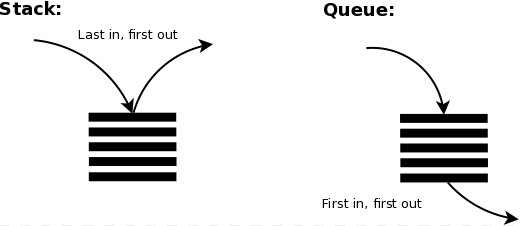
\includegraphics[width=10cm]{figures/FIFO_LIFO.png}
					\caption{Stacks and queues
					\scriptsize{ (source: Martin Franěk, \url{quora.com})}}
				\end{center}
			\end{figure}

		\subsection{Object oriented programming}

			\subsubsection{Definition}
				Some data types can handle references to different primitive variables in a common data structure. These variables are usually called \textbf{attributes}.
				\textbf{Object Oriented Programming} makes possible to define these types using \textbf{
		classes}. Each variable built from a class is called an \textbf{object}. It interacts with other variables through \textbf{methods}.
				\textbf{Inheritance} makes it possible for such a custom data type (\textit{T2}) to have the properties (attributes, methods) of another one (\textit{T1}).

			\subsubsection{Examples}

				\paragraph{First}
					We can think about an \textbf{Official identity} type that stores the following information:
					\begin{itemize}
							\item Unique identifier: \textit{Int}
							\item Name: \textit{String}
							\item Height: \textit{Float16}
							\item Parent(s) and siblings: containers of objects of type \textit{Official identity}
					\end{itemize}
					One could also partly define \textbf{Official identity} from a type \textbf{Identity} (inheritance):
					\begin{itemize}
							\item Name: \textit{String}
					\end{itemize}
					In that case, the \textquote{Name} attributed would be inherited from the parent object of type \textbf{Identity}. Then \textbf{Official identity} specifies 
                    \textbf{Identity}: every property of \textbf{Identity} is a property of \textbf{Official identity} (but not the other way).

				\paragraph{Second}
					In case of onheritance, one can \textbf{overload} some methods of the parent (see \textit{park} in the example below)
					\begin{figure}[h!]
							\centering
							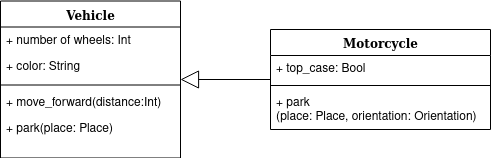
\includegraphics[width=10cm]{figures/Heritage/Heritage.drawio.png}
							\caption{Inheritance as a UML description}
					\end{figure}

		\section{Variable scope}

			\subsection{Definition}
				Each language defines different variable scope rules. These rules state whether a variable created in a scope A can be accessed from a scope B. 
                These rules are related to:
				\begin{itemize}
					\item Control flow structures
					\item Functions
					\item Local code imports
					\item \ldots
				\end{itemize}
				These rules makes it possible to use a common variable name in different places in the code, to refer to different variables.
                \textbf{Shadowing} refers to the fact of reusing for a different purpose an already defined variable name

			\subsection{Static and dynamic typing}
				Static typing consists in the manual assignment of a type to a variable. This variable will keep this type until the end of its use.
				Dynamic typing let the compiler (or interpreter) chose the variable type during run time. \\
				In both cases, the variable has a known type during execution.

		\section{Mutability}
        		The mutability of an object refers to the possibility of modifying its properties.

			\subsection{Copy and assignment}
				The assignment of a mutable object to another variable might lead to unexpected results. Indeed:
\begin{itemize}
\item The in-depth copy of an object makes a full duplicate of this object.
				(Figure \ref{fig:copie}). 
\item Conversely, an assignment of a mutable object to a variable makes the variable reference the memory content of the object (Figure \ref{fig:vue}).
    \end{itemize}
				 In the first case, a modification on the first variable has no effect on the second. In the second case, if first is modified then second is modified too.
				 \\
				 \textbf{There exists an intermediate copy level between assignment and in-depth copy}: shallow copy. If 'b' is a shallow copy of 'a', 'b' has a different memory address than 'a' (different objects), yet references of 'b' to mutables objects are the one of 'a'. 

				\begin{figure}[h!]
					\centering
					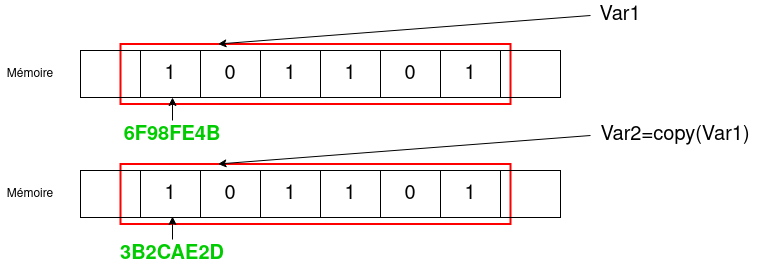
\includegraphics[width=15cm]{figures/Mutabilite/Mutabilite - copie.drawio}
					\caption{In-depth copy of a variable}
					\label{fig:copie}
				\end{figure}
				\begin{figure}[h!]
					\centering
					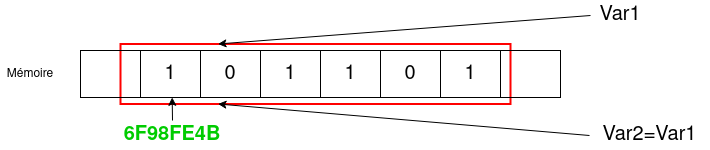
\includegraphics[width=15cm]{figures/Mutabilite/Mutabilite - vue.drawio}
					\caption{Reference to a variable}
					\label{fig:vue}
				\end{figure}

			\subsection{Equality and identity}
				Some objects can be equal - i.e. same properties - withouth being the same - i.e. different memory address. 
            The identity test makes it possible to check if 2 objets have the same identity. Using pseudo-code:

	\begin{verbatim}
		MyType var1 = MyType.constructor()
		MyType var2 = InDepthCopy(var1)
		AreIdentical(var1, var2)  # False
		AreEqual(var1, var2)  	  # True
				\end{verbatim}

\end{document}
